\let\negmedspace\undefined
\let\negthickspace\undefined

\documentclass[journal,12pt,twocolumn]{IEEEtran}
%\documentclass[journal,12pt,twocolumn]{IEEEtran}
%
\usepackage{setspace}
\usepackage{gensymb}
%\doublespacing
\singlespacing
\renewcommand{\thefigure}{\theenumi}
%\usepackage{graphicx}
%\usepackage{amssymb}
%\usepackage{relsize}
\usepackage[cmex10]{amsmath}
%\usepackage{amsthm}
%\interdisplaylinepenalty=2500
%\savesymbol{iint}
%\usepackage{txfonts}
%\restoresymbol{TXF}{iint}
%\usepackage{wasysym}
\usepackage{amsthm}
\usepackage{mathrsfs}
\usepackage{txfonts}
\usepackage{stfloats}
\usepackage{cite}
\usepackage{cases}
\usepackage{subfig}
%\usepackage{xtab}
\usepackage{longtable}
\usepackage{multirow}
%\usepackage{algorithm}
%\usepackage{algpseudocode}
\usepackage{enumitem}
\usepackage{mathtools}
\usepackage{tikz}
\usepackage{circuitikz}
\usepackage{verbatim}
\usepackage{hyperref}
%\usepackage{stmaryrd}
\usepackage{tkz-euclide} % loads  TikZ and tkz-base
%\usetkzobj{all}
\usepackage{listings}
    \usepackage{color}                                            %%
    \usepackage{array}                                            %%
    \usepackage{longtable}                                        %%
    \usepackage{calc}                                             %%
    \usepackage{multirow}                                         %%
    \usepackage{hhline}                                           %%
    \usepackage{ifthen}                                           %%
  %optionally (for landscape tables embedded in another document): %%
    \usepackage{lscape}     
\usepackage{multicol}
\usepackage{chngcntr}
\usepackage{iftex}
%\usepackage[latin9]{inputenc}
\usepackage{geometry}
\usepackage{bm}
%\geometry{verbose,tmargin=2cm,bmargin=3cm,lmargin=1.8cm,rmargin=1.5cm,headheight=2cm,headsep=2cm,footskip=3cm}
\usepackage{array}
\newcolumntype{L}[1]{>{\raggedright\let\newline\\\arraybackslash\hspace{0pt}}m{#1}}
\newcolumntype{C}[1]{>{\centering\let\newline\\\arraybackslash\hspace{0pt}}m{#1}}
\newcolumntype{R}[1]{>{\raggedleft\let\newline\\\arraybackslash\hspace{0pt}}m{#1}}

%\usepackage{graphicx}
%\usepackage{setspace}
%\usepackage{parskip}

\def \hsp {\hspace{3mm}}

\makeatletter

\providecommand{\tabularnewline}{\\}



\makeatother
\ifxetex
\usepackage[T1]{fontenc}
\usepackage{fontspec}
%\setmainfont[ Path = fonts/]{Sanskrit_2003.ttf}
\newfontfamily\nakulafont[Script=Devanagari,AutoFakeBold=2,Path = fonts/]{Nakula}
%\newfontfamily\liberationfont{Liberation Sans Narrow}
%\newfontfamily\liberationsansfont{Liberation Sans}
\fi
\usepackage{tikz}
\usepackage{xcolor}
%\usepackage{enumerate}

%\usepackage{wasysym}
%\newcounter{MYtempeqncnt}
\DeclareMathOperator*{\Res}{Res}
%\renewcommand{\baselinestretch}{2}
\renewcommand\thesection{\arabic{section}}
\renewcommand\thesubsection{\thesection.\arabic{subsection}}
\renewcommand\thesubsubsection{\thesubsection.\arabic{subsubsection}}

\renewcommand\thesectiondis{\arabic{section}}
\renewcommand\thesubsectiondis{\thesectiondis.\arabic{subsection}}
\renewcommand\thesubsubsectiondis{\thesubsectiondis.\arabic{subsubsection}}

% correct bad hyphenation here
\hyphenation{op-tical net-works semi-conduc-tor}
\def\inputGnumericTable{}                                 %%

\lstset{
language=tex,
frame=single, 
breaklines=true
}

%\begin{document}
%


\newtheorem{theorem}{Theorem}[section]
\newtheorem{problem}{Problem}
\newtheorem{proposition}{Proposition}[section]
\newtheorem{lemma}{Lemma}[section]
\newtheorem{corollary}[theorem]{Corollary}
\newtheorem{example}{Example}[section]
\newtheorem{definition}[problem]{Definition}
%\newtheorem{thm}{Theorem}[section] 
%\newtheorem{defn}[thm]{Definition}
%\newtheorem{algorithm}{Algorithm}[section]
%\newtheorem{cor}{Corollary}
\newcommand{\BEQA}{\begin{eqnarray}}
\newcommand{\EEQA}{\end{eqnarray}}
\newcommand{\define}{\stackrel{\triangle}{=}}
\bibliographystyle{IEEEtran}
%\bibliographystyle{ieeetr}
\providecommand{\mbf}{\mathbf}
\providecommand{\pr}[1]{\ensuremath{\Pr\left(#1\right)}}
\providecommand{\qfunc}[1]{\ensuremath{Q\left(#1\right)}}
\providecommand{\sbrak}[1]{\ensuremath{{}\left[#1\right]}}
\providecommand{\lsbrak}[1]{\ensuremath{{}\left[#1\right.}}
\providecommand{\rsbrak}[1]{\ensuremath{{}\left.#1\right]}}
\providecommand{\brak}[1]{\ensuremath{\left(#1\right)}}
\providecommand{\lbrak}[1]{\ensuremath{\left(#1\right.}}
\providecommand{\rbrak}[1]{\ensuremath{\left.#1\right)}}
\providecommand{\cbrak}[1]{\ensuremath{\left\{#1\right\}}}
\providecommand{\lcbrak}[1]{\ensuremath{\left\{#1\right.}}
\providecommand{\rcbrak}[1]{\ensuremath{\left.#1\right\}}}
\theoremstyle{remark}
\newtheorem{rem}{Remark}
\newcommand{\sgn}{\mathop{\mathrm{sgn}}}
\providecommand{\abs}[1]{\left\vert#1\right\vert}
\providecommand{\res}[1]{\Res\displaylimits_{#1}} 
\providecommand{\norm}[1]{\left\lVert#1\right\rVert}
%\providecommand{\norm}[1]{\lVert#1\rVert}
\providecommand{\mtx}[1]{\mathbf{#1}}
\providecommand{\mean}[1]{E\left[ #1 \right]}
\providecommand{\fourier}{\overset{\mathcal{F}}{ \rightleftharpoons}}
%\providecommand{\hilbert}{\overset{\mathcal{H}}{ \rightleftharpoons}}
%\providecommand{\system}{\overset{\mathcal{H}}{ \longleftrightarrow}}
\providecommand{\system}[1]{\overset{\mathcal{#1}}{ \longleftrightarrow}}
\providecommand{\gauss}[2]{\mathcal{N}\ensuremath{\left(#1,#2\right)}}
%
	%\newcommand{\solution}[2]{\textbf{Solution:}{#1}}
\newcommand{\solution}{\noindent \textbf{Solution: }}
\newcommand{\cosec}{\,\text{cosec}\,}
\newcommand{\sinc}{\,\text{sinc}\,}
\newcommand{\rect}{\,\text{rect}\,}
\providecommand{\dec}[2]{\ensuremath{\overset{#1}{\underset{#2}{\gtrless}}}}
\newcommand{\myvec}[1]{\ensuremath{\begin{pmatrix}#1\end{pmatrix}}}
\newcommand{\mydet}[1]{\ensuremath{\begin{vmatrix}#1\end{vmatrix}}}
\newcommand*{\permcomb}[4][0mu]{{{}^{#3}\mkern#1#2_{#4}}}
\newcommand*{\perm}[1][-3mu]{\permcomb[#1]{P}}
\newcommand*{\comb}[1][-1mu]{\permcomb[#1]{C}}
%\numberwithin{equation}{section}
\numberwithin{equation}{section}
%\numberwithin{problem}{section}
%\numberwithin{definition}{section}
\makeatletter
\@addtoreset{figure}{problem}
\makeatother
\let\StandardTheFigure\thefigure
\let\vec\mathbf
%\renewcommand{\thefigure}{\theproblem.\arabic{figure}}
\renewcommand{\thefigure}{\theproblem}
%\setlist[enumerate,1]{before=\renewcommand\theequation{\theenumi.\arabic{equation}}
%\counterwithin{equation}{enumi}
%\renewcommand{\theequation}{\arabic{subsection}.\arabic{equation}}
\vspace{3cm}
%\usepackage{babel}
\begin{document}
\title{Probability and Random Variables\\Assignment}
\author{Shreyas Wankhede}
\maketitle

\section{Uniform Random Numbers}
Let $U$ be a uniform random variable between 0 and 1.
\begin{enumerate}[label=\thesection.\arabic*
,ref=\thesection.\theenumi]
\item Generate $10^6$ samples of $U$ using a C program and save into a file called uni.dat .
\\
\solution Download the following files and execute the  C program.
\begin{lstlisting}
wget https://github.com/shreyaswankhede12/Random_numbers/blob/main/codes/1.1_exrand.
wget https://github.com/shreyaswankhede12/Random_numbers/blob/main/codes/coeffs.h
\end{lstlisting}
Compile and run the C program by executing the following
\begin{lstlisting}
cc -lm 1.1_exrand.c
./a.out
\end{lstlisting}
%
\item
Load the uni.dat file into python and plot the empirical CDF of $U$ using the samples in uni.dat. The CDF is defined as
\begin{align}
F_{U}(x) = \pr{U \le x}
\end{align}
\solution  Download the following Python code that plots
\begin{lstlisting}
wget https://github.com/shreyaswankhede12/Random_numbers/blob/main/codes/1.2_cdf.py
\end{lstlisting}
Run the code by executing
\begin{lstlisting}
python 1.2_cdf.py
\end{lstlisting}
\begin{figure}
\centering
\includegraphics[width=\columnwidth]{1.2_FIG.pdf}
Fig:1.2 CDF of U
\end{figure}
%
\item
Find a  theoretical expression for $F_{U}(x)$.
\solution The PDF of $U$ is given by
	\begin{align}
		p_{U}(x) = 
		\begin{cases}
			1 & x \in [0, 1] \\
			0 & \text{otherwise}
		\end{cases}
	\end{align}
	
	The CDF of $U$ is given by
	\begin{align}
		F_{U}(x) = \pr{U \le x} = \int_{-\infty}^x p_{U}(x) ~\mathrm{d}x
	\end{align}
	
	If $x<0$,
	\begin{align}
		\int_{-\infty}^x p_{U}(x) ~\mathrm{d}x = \int_{-\infty}^x 0 ~\mathrm{d}x = 0
	\end{align}
	
	If $c$,
	\begin{align}
		\int_{-\infty}^x p_{U}(x) ~\mathrm{d}x &= \int_{-\infty}^0 0 ~\mathrm{d}x + \int_0^x 1 ~\mathrm{d}x \\
		&= 0 + x \\
		&= x
	\end{align}
	
	If $x>1$,
	\begin{multline}
		\int_{-\infty}^x p_{U}(x) ~\mathrm{d}x \\= \int_{-\infty}^0 0 ~\mathrm{d}x + \int_0^1 1 ~\mathrm{d}x +  \int_1^x 0 ~\mathrm{d}x 
	\end{multline}
	\begin{align}
		\int_{-\infty}^x p_{U}(x) ~\mathrm{d}x &= 0 + 1 + 0 \\
		&= 1
	\end{align}
	
	Therefore, we obtain the CDF of $U$ as
	\begin{align}
		F_{U}(x) = 
		\begin{cases}
			0 & x < 0 \\
			x & 0 \le x \le 1 \label{eq:1.11}\\
			1 & x > 1
		\end{cases}
	\end{align}
\item
The mean of $U$ is defined as
%
\begin{equation}
E\sbrak{U} = \frac{1}{N}\sum_{i=1}^{N}U_i
\end{equation}
%
and its variance as
%
\begin{equation}
\text{var}\sbrak{U} = E\sbrak{U- E\sbrak{U}}^2 
\end{equation}
Write a C program to  find the mean and variance of $U$. \\
\solution execute the following
\begin{lstlisting}
wget https://github.com/shreyaswankhede12/Random_numbers/blob/main/codes/1.4.c
\end{lstlisting}
\item Verify your result theoretically given that
\end{enumerate}
%
\begin{equation}
E\sbrak{U^k} = \int_{-\infty}^{\infty}x^kdF_{U}(x)
\end{equation}\\
\textbf{solution:}From 1.11,
\begin{align}
F_{U}(X)&=x \hspace{3mm}\forall x, 0\leq x\leq 1\nonumber\\
\therefore dF_{U}(X)&=dx\\
E[U]&=\int_{0}^{1}xdx=\dfrac{1}{2}=0.5
\end{align}
similarly,
\begin{align}
E[U^2]&=\int_{0}^{1}x^2dx=\dfrac{1}{3}\\
Var[U]&=E[U^2]-(E[U])^2\\
&=\dfrac{1}{3}-\Big(\dfrac{1}{2}\Big)^2\nonumber\\
&=\dfrac{1}{3}-\dfrac{1}{4}\nonumber\\
&=\dfrac{1}{12}\nonumber
\end{align}

\section{Central Limit Theorem}
%
\begin{enumerate}[label=\thesection.\arabic*
,ref=\thesection.\theenumi]
%
\item
Generate $10^6$ samples of the random variable
%
\begin{equation}
X = \sum_{i=1}^{12}U_i -6
\end{equation}
%
using a C program, where $U_i, i = 1,2,\dots, 12$ are  a set of independent uniform random variables between 0 and 1
and save in a file called gau.dat
\solution link for the code:
\begin{lstlisting}
wget https://github.com/shreyaswankhede12/Random_numbers/blob/main/codes/2.1.c\\
wget https://github.com/shreyaswankhede12/Random_numbers/blob/main/codes/coeffs.h
\end{lstlisting}
execute the following by
\begin{lstlisting}
gcc 2.1.c -lm\\
./a.out
\end{lstlisting}
\item
Load gau.dat in python and plot the empirical CDF of $X$ using the samples in gau.dat. What properties does a CDF have?
\\
\solution The CDF of $X$ is plotted 
link to the python code
\begin{lstlisting}
wget https://github.com/shreyaswankhede12/Random_numbers/blob/main/codes/2.2_emp_cdf.py
\end{lstlisting}
execute the following by
\begin{lstlisting}
python 2.2_emp_cdf.py
\end{lstlisting}
\begin{figure}
\centering
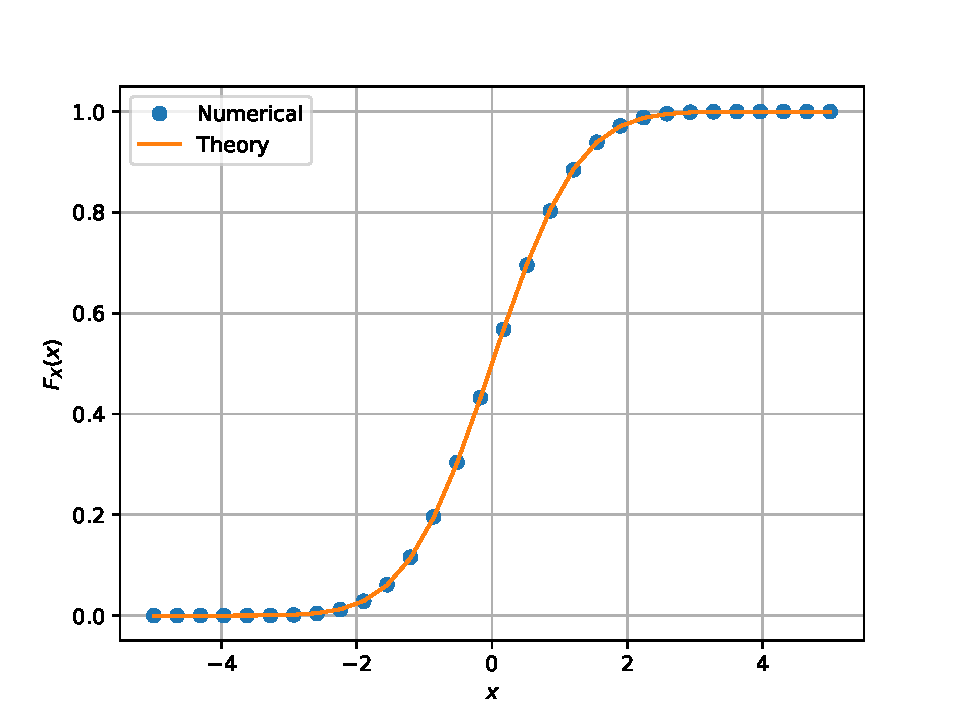
\includegraphics[width=\columnwidth]{2.2.pdf}
Fig:2.2 The CDF of X
\end{figure}
\item
Load gau.dat in python and plot the empirical PDF of $X$ using the samples in gau.dat. The PDF of $X$ is defined as
\begin{align}
p_{X}(x) = \frac{d}{dx}F_{X}(x)
\end{align}
What properties does the PDF have?
\\
\solution The PDF of $X$ is plotted in Fig. 2.3 using the code below
\begin{lstlisting}
wget https://github.com/shreyaswankhede12/Random_numbers/blob/main/codes/2.3_emp_pdf.py
\end{lstlisting}
\begin{figure}
\centering
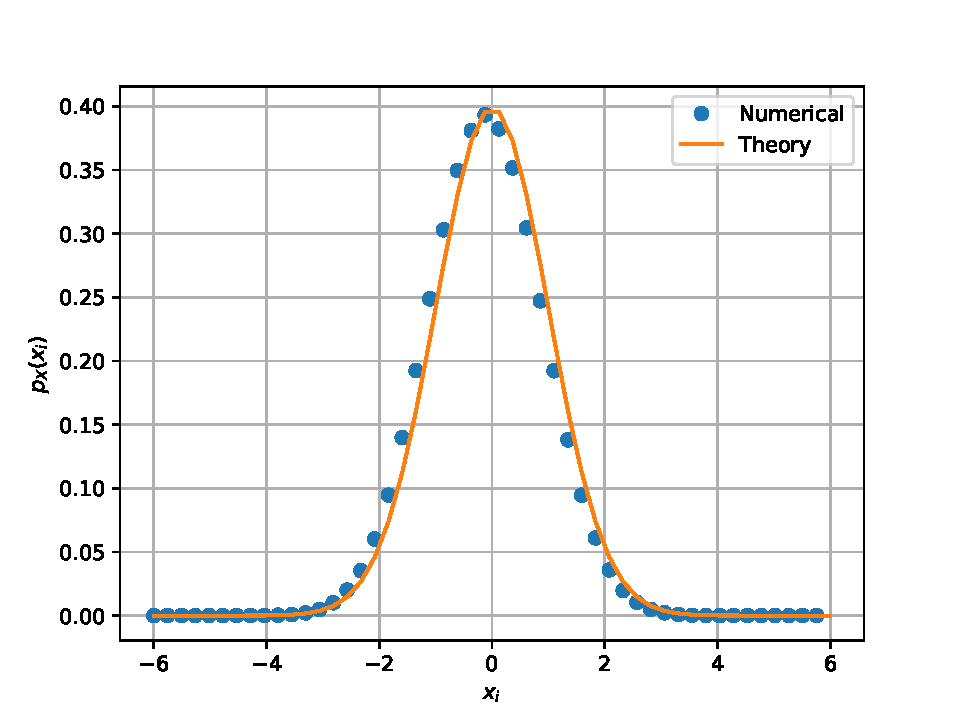
\includegraphics[width=\columnwidth]{2.3.pdf}
Fig:2.3  The PDF of X
\end{figure}
\item Find the mean and variance of $X$ by writing a C program.\\
\solution link for c program
\begin{lstlisting}
wget https://github.com/shreyaswankhede12/Random_numbers/blob/main/codes/2.4.c
\end{lstlisting}
execute the following by
\begin{lstlisting}
gcc 2.4.c -lm
\end{lstlisting}
\item Given that 
\begin{align}
p_{X}(x) = \frac{1}{\sqrt{2\pi}}\exp\brak{-\frac{x^2}{2}}, -\infty < x < \infty,
\end{align}
repeat the above exercise theoretically.
\end{enumerate}
\textbf{solution:}
\begin{align}
E[X]&=\int_{-\infty}^{\infty}xP_{X}(x)dx\\
&=\int_{-\infty}^{\infty}\dfrac{x}{\sqrt{2\pi}}\exp\brak{\dfrac{-x^2}{2}}dx\\
\text{Let}\hspace{2mm} h(x)&=\dfrac{x}{\sqrt{2\pi}}\exp\brak{\dfrac{-x^2}{2}}\nonumber
\end{align}
Now,
\begin{align}
h(-x)=-h(x)\nonumber
\end{align}
Thus h(x) is an odd function
\begin{align}
\therefore E[X]&=\int_{-\infty}^{\infty}h(x)dx=0\\
E[X^2]&=\int_{-\infty}^{\infty}x^2P_{X}(x)dx\\
&=\int_{-\infty}^{\infty}\dfrac{x^2}{\sqrt{2\pi}}\exp\brak{\dfrac{-x^2}{2}}dx
\end{align}
Using integration by parts:
  \begin{align}
   \label{eq:eq1}
 & =x\int xe^{\frac{-x^2}{2}} dx-\int\frac{d(x)}{dx} \int xe^{\frac{-x^2}{2}}dx\\
 &I=\int x e^{\frac{-x^2}{2}}\\
 &\text{Let}\hspace{2mm}  \frac{x^2}{2}=t \\
 &\implies x dx=dt\\
 &\implies \int e^{-t} dt=-e^{-t} +c\\
 \label{eq:eq2}
 &\therefore \int x e^{\frac{-x^2}{2}}=-e^{\frac{-x^2}{2}} +c
 \end{align}
 Using \eqref{eq:eq2} in \eqref{eq:eq1}
 \begin{align}
&= -x e^{\frac{-x^2}{2}}+\int e^{\frac{-x^2}{2}} dx\\
&\text{Also} ,\int_{-\infty}^{\infty} e^{\frac{-x^2}{2}} dx=\sqrt{2 \pi} 
\end{align}
$\therefore$ substituting limits we get
\begin{align}
 E[x^2]&=1\\
 \text{var}(X)&=E[x^2]-(E[x])^2=1-0
\end{align}
 
\section{From Uniform to Other}
\begin{enumerate}[label=\thesection.\arabic*
,ref=\thesection.\theenumi]
%
\item
Generate samples of 
%
\begin{equation}
V = -2\ln\brak{1-U}
\end{equation}
%
and plot its CDF. \\
\solution: Run the following codes
\begin{lstlisting}
wget https://github.com/shreyaswankhede12/Random_numbers/blob/main/codes/3.1_code.c
\end{lstlisting}
execute by commands:
\begin{lstlisting}
gcc 3.1_code.c -lm
./a.out
\end{lstlisting}
\begin{lstlisting}
wget https://github.com/shreyaswankhede12/Random_numbers/blob/main/codes/3.1_plot.py
\end{lstlisting}
\begin{figure}
\centering
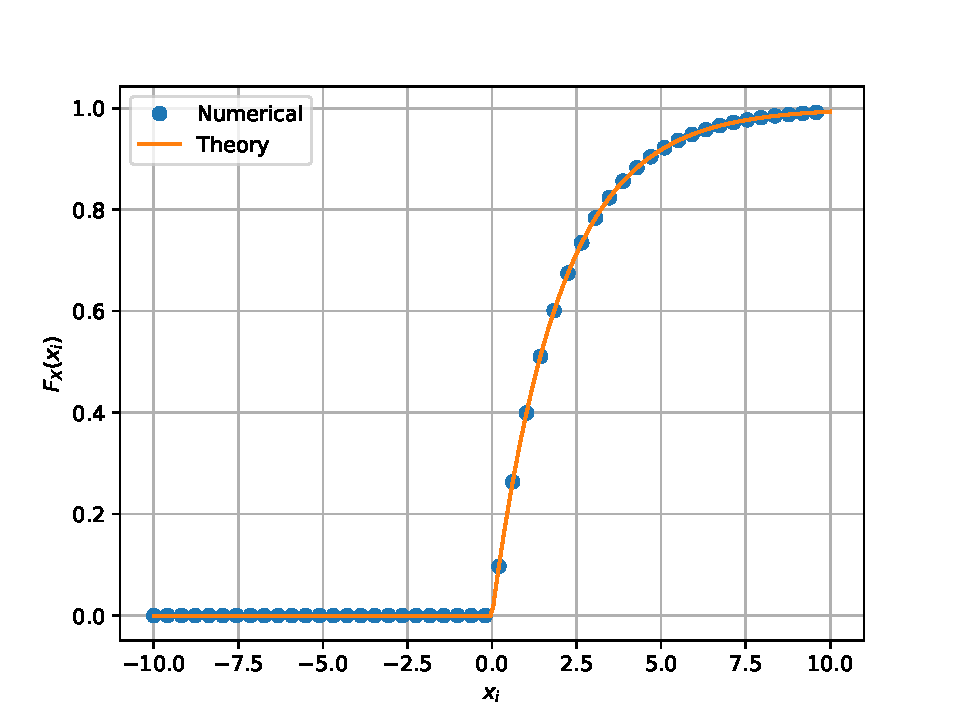
\includegraphics[width=\columnwidth]{3.1.pdf}
Fig:3.1  The CDF of V
\end{figure}
\item Find a theoretical expression for $F_V(x)$.
\solution We have
	\begin{align}
		F_V(x) &= \pr{V \le x} \\
		&= \pr{-2\ln\brak{1-U} \le x} \\
		&= \pr{\ln\brak{1-U} \ge -\frac{x}{2}} \\
		&= \pr{1-U \ge \exp\brak{-\frac{x}{2}}} \\
		&= \pr{U \le 1 - \exp\brak{-\frac{x}{2}}} \\
		&= F_U\brak{1 - \exp\brak{-\frac{x}{2}}}
	\end{align}
	Now,
	\begin{align}
		0 \le 1-\exp\brak{-\frac{x}{2}} &< 1 \qquad \text{if } x \ge 0	\\	
		1-\exp\brak{-\frac{x}{2}} &< 0 \qquad \text{if } x < 0	
	\end{align}
	
	Therefore, from \eqref{eq:1.11}
	\begin{align}
		F_V(x) = 
		\begin{cases}
			1-\exp\brak{-\dfrac{x}{2}} & x \ge 0 \\
			0 & x < 0
		\end{cases}
	\end{align}
%
%\item
%Generate the Rayleigh distribution from Uniform. Verify your result through graphical plots.
\end{enumerate}
\section{Triangular Distribution}
\begin{enumerate}[label=\thesection.\arabic*
,ref=\thesection.\theenumi]
%
\item Generate 
	\begin{align}
		T = U_1+U_2
	\end{align}
\solution
this generates $U_1$ and $U_2$
\begin{lstlisting}
wget https://github.com/shreyaswankhede12/Random_numbers/blob/main/codes/4.1_gen_u1_u2.c
\end{lstlisting}
this code generates $U_1 + U_2$
\begin{lstlisting}
wget https://github.com/shreyaswankhede12/Random_numbers/blob/main/codes/4.1_gen_u1+u2.c
\end{lstlisting} 
\item Find the CDF of $T$.\\
\solution python code for plotting cdf:
\begin{lstlisting}
wgethttps://github.com/shreyaswankhede12/Random_numbers/blob/main/codes/4.2.py
\end{lstlisting}
\begin{figure}
\centering
\includegraphics[width=\columnwidth]{4.2.pdf}
Fig:4.2  The CDF of T
\end{figure}
\item Find the PDF of $T$.\\
\solution python code for plotting pdf:
\begin{lstlisting}
wget https://github.com/shreyaswankhede12/Random_numbers/blob/main/codes/4.3.py
\end{lstlisting}
\begin{figure}
\centering
\includegraphics[width=\columnwidth]{4.3.pdf}
Fig:4.3  The PDF of T
\end{figure} 
\item Find the theoretical expressions for the PDF and CDF of $T$.\\
\solution The CDF of $T$ is given by
	\begin{align}
		F_T(t) = \pr{T \le t} = \pr{U_1 + U_2 \le t}	
	\end{align}		
	$ U_1 + U_2 \in [0,2]$\\
	Thus, for $t \ge 2$, then $U_1 + U_2 \le t$ is always true\\  for $t < 0$, then $U_1 + U_2 \le t$ is always false.
	
	Now, fix the value of $U_1$ to be some $x$
	\begin{align}
		x + U_2 \le t \implies U_2 \le t - x
	\end{align}
	
	If $0 \le t \le 1$, then $x$ can take all values in $[0,t]$
	\begin{align}
		F_T(t)	=\int_0^t F_{U_2}(t-x) p_{U_1}(x) dx 
	\end{align}
	since,\hspace{3mm}$t-x \in [0,1]$
	\begin{align}
		F_{U_2}(t-x)=t-x
	\end{align}
	\begin{align}
		F_T(t) &= \int_0^t (t-x) . 1 . dx \\
		&= \frac{t^2}{2}
	\end{align}
	
	If $1 < t < 2$, $x$ can only take values in $[0,1]$ as $U_1 \le 1$
	\begin{align}
		F_T(t)	&= \int_0^1 F_{U_2}(t-x) . 1 . dx 
	\end{align}
	since, \hspace{3mm} $t-x \in [0,1],$
	\begin{align}
		F_T(t) &= \int_0^{t-1} 1 dx + \int_{t-1}^1 (t-x)dx \\ 
		&= -\frac{t^2}{2} + 2t - 1
	\end{align}
	
	Therefore,
	\begin{align}
		F_T(t) = 
		\begin{cases}
		0 & t < 0 \\
		\dfrac{t^2}{2} & 0 \le t \le 1 \\
		 2t -\dfrac{t^2}{2} - 1 & 1 < t < 2 \\
		1 & t \ge 2
		\end{cases}
	\end{align}
	On differentiating, we get,\\
	\begin{align}
		P_T(t) = 
		\begin{cases}
		0 & t < 0 \\
		t & 0 \le t \le 1 \\
		 2-t & 1 < t < 2 \\
		1 & t \ge 2
		\end{cases}
	\end{align}
\item Verify your results through a plot. \\
\solution Refer to solution of qs 4.2 and 4.3
\end{enumerate}
\section{Maximul Likelihood}
\begin{enumerate}[label=\thesection.\arabic*
,ref=\thesection.\theenumi]
\item Generate 
\begin{equation}
Y = AX+N,
\end{equation}
		where $A = 5 \text{ dB}, X \i \cbrak{1,-1}$,  is Bernoulli and $N \sim \gauss{0}{1}$.
	\item Plot $Y$.
	\item Guess how to estimate $X$ from $Y$.
\item
\label{ml-ch4_sim}
Find 
\begin{equation}
	P_{e|0} = \pr{\hat{X} = -1|X=1}
\end{equation}
and 
\begin{equation}
	P_{e|1} = \pr{\hat{X} = 1|X=-1}
\end{equation}
%
\item Find $P_e$.
%
\item
Verify by plotting  the theoretical $P_e$.  
		\end{enumerate}
\section{Gaussian to Other}
\begin{enumerate}[label=\thesection.\arabic*
,ref=\thesection.\theenumi]
\item
Let $X_1 \sim  \gauss{0}{1}$ and $X_2 \sim  \gauss{0}{1}$. Plot the CDF and PDF of
%
\begin{equation}
V = X_1^2 + X_2^2
\end{equation}
%
%
%
\item
If
%
\begin{equation}
F_{V}(x) = 
\begin{cases}
1 - e^{-\alpha x} & x \geq 0 \\
0 & x < 0,
\end{cases}
\end{equation}
%
find $\alpha$.
%
\item
\label{ch3_raleigh_sim}
Plot the CDF and PDf of
%
\begin{equation}
A = \sqrt{V}
\end{equation}
%
\end{enumerate}
\section{Conditional Probability}
\begin{enumerate}[label=\thesection.\arabic*
,ref=\thesection.\theenumi]
\item
\item
\label{ch4_sim}
Plot 
\begin{equation}
P_e = \pr{\hat{X} = -1|X=1}
\end{equation}
%
for 
\begin{equation}
Y = AX+N,
\end{equation}
where $A$ is Raleigh with $E\sbrak{A^2} = \gamma, N \sim \gauss{0}{1}, X \in \brak{-1,1}$ for $0 \le \gamma \le 10$ dB.
%
\item
Assuming that $N$ is a constant, find an expression for $P_e$.  Call this $P_e(N)$
%
\item
%
\label{ch4_anal}
For a function $g$,
\begin{equation}
E\sbrak{g(X)} = \int_{-\infty}^{\infty}g(x)p_{X}(x)\, dx
\end{equation}
%
Find $P_e = E\sbrak{P_e(N)}$.
%
\item
Plot $P_e$ in problems \ref{ch4_sim} and \ref{ch4_anal} on the same graph w.r.t $\gamma$.  Comment.
		\end{enumerate}
\section{Two Dimensions}
Let 
\begin{equation}
\mbf{y} = A\mbf{x} + \mbf{n},
\end{equation}
where 
\begin{align}
x &\in \brak{\mbf{s}_0,\mbf{s}_1}, 
\mbf{s}_0 = 
\begin{pmatrix}
1 
\\
0
\end{pmatrix},
\mbf{s}_1 = 
\begin{pmatrix}
0 
\\
1
\end{pmatrix}
\\
\mbf{n} &= 
\begin{pmatrix}
n_1
\\
n_2
\end{pmatrix},
n_1,n_2 \sim \gauss{0}{1}.
\end{align}
%
\begin{enumerate}[label=\thesection.\arabic*
,ref=\thesection.\theenumi]
%%
\item
\label{ch5_fsk}
Plot 
%
\begin{equation}
\mbf{y}|\mbf{s}_0 \text{ and } \mbf{y}|\mbf{s}_1
\end{equation}
%
on the same graph using a scatter plot.
%
\item
For the above problem, find a decision rule for detecting the symbols $\mbf{s}_0 $ and $\mbf{s}_1$.
%
\item
Plot 
\begin{equation} 
P_e = \pr{\hat{\mbf{x}} = \mbf{s}_1|\mbf{x} = \mbf{s}_0}
\end{equation}
with respect to the SNR from 0 to 10 dB.
%
\item
Obtain an expression for $P_e$. Verify this by comparing the theory and simulation plots on the same graph.
%
		\end{enumerate}
\end{document}